\documentclass[11pt]{article}
\usepackage[a4paper,left=1.5cm,right=1.5cm,top=1.5cm,bottom=1.5cm]{geometry}
\usepackage{fancyhdr}
\usepackage{mleftright}
\usepackage{verbatim}
\renewcommand{\headrulewidth}{1pt}
\fancyhead[C]{\textsc{[LINMA2380] --- Homework 2}}
\fancyhead[L]{2 November 2020}
\fancyhead[R]{Group 02}

\usepackage{tikz}
\usepackage{pgfplots}
\usepackage[T1]{fontenc}
\usepackage[utf8]{inputenc}
\usepackage[english]{babel}
\usepackage{graphicx}
\usepackage{subcaption}
\usepackage{csquotes}
\usepackage{mathtools,amssymb,amsthm}
\usepackage[binary-units=true,separate-uncertainty = true,multi-part-units=single]{siunitx}
\usepackage{float}
\usepackage[linktoc=all]{hyperref}
\hypersetup{breaklinks=true}
\graphicspath{{img/}}
\usepackage{caption}
\usepackage{textcomp}
\usepackage{array}
\usepackage{color}
\usepackage{tabularx,booktabs}
\usepackage{titlesec}
\usepackage{wrapfig}
\pagestyle{fancy}
\usepackage{mathrsfs}
\usepackage{bm}
\DeclarePairedDelimiterX{\norm}[1]{\lVert}{\rVert}{#1}

\newcommand{\imag}{\mathrm{i}\mkern1mu} % Imaginary unit
\newcommand{\abs}[1]{\left\lvert#1\right\lvert}
\usepackage{listings}
\lstset{
	language=Python,
	numbers=left,
	numberstyle=\tiny\color{gray},
	basicstyle=\rm\small\ttfamily,
	keywordstyle=\bfseries\color{dkred},
	frame=single,
	commentstyle=\color{gray}=small,
	stringstyle=\color{dkgreen},
	%backgroundcolor=\color{gray!10},
	%tabsize=8, % Thank you Papa Torvalds
	%rulecolor=\color{black!30},
	%title=\lstname,
	breaklines=true,
	framextopmargin=2pt,
	framexbottommargin=2pt,
	extendedchars=true,
	inputencoding=utf8,
}

\DeclareMathOperator*{\argmin}{arg\,min}

\DeclareMathOperator{\rank}{rank}
\DeclareMathOperator{\Ker}{Ker}
\DeclareMathOperator{\vect}{vec}
\DeclareMathOperator{\newdiff}{d} % use \dif instead
\newcommand{\dif}{\newdiff\!}
\newcommand{\e}{\mathrm{e}}

\newcommand{\field}{\mathbb{F}} % field
\newcommand{\real}{\mathbb{R}} % real numbers
\newcommand{\complex}{\mathbb{C}} % complex numbers

\newcommand{\snorm}[1]{\norm{#1}_2} % spectral norm
\newcommand{\fnorm}[1]{\norm{#1}_F} % frobenius norm

\setcounter{MaxMatrixCols}{15}

\newcommand\undermat[2]{% http://tex.stackexchange.com/a/102468/5764
	\makebox[0pt][l]{$\smash{\underbrace{\phantom{%
					\begin{matrix}#2\end{matrix}}}_{\text{$#1$}}}$}#2}

\begin{document}
\section*{Exercise A: Least square problems}
\subsection*{A1}
\begin{proof}
	Minimising $\snorm{Ax - b}$ with respect to \(x\) means finding \(x\) such that the derivative of $\snorm{Ax - b}$ with respect to \(x\) is equal to zero.
	Equivalently, we can minimise the square of the norm which can be developed as follows:
	\begin{align*}
	\snorm{Ax - b}^2 &= \snorm{Ax}^2 - 2 \langle Ax,b \rangle + \snorm{b}^2 \\
	&= x^\top A^\top Ax - 2x^\top A^\top b + b^\top b. 
	\end{align*}
	The derivative of this expression with respect to \(x\) is
	\begin{align*}
	\frac{\partial \snorm{Ax - b}^2}{\partial x} &= \frac{\partial(x^\top A^\top Ax - 2x^\top A^\top b + b^\top b)}{\partial x} \\
	&= \frac{\partial(x^\top A^\top Ax)}{\partial x} - \frac{\partial(2x^\top A^\top b)}{\partial x} + \frac{\partial(b^\top b)}{\partial x} \\
	&= 2A^\top Ax - 2A^\top b + 0.
	\end{align*}
	We set this derivative to zero to obtain the following:
	\begin{align*}
	\frac{\partial \snorm{Ax - b}^2}{\partial x} = 0\\
	\iff 2A^\top Ax - 2A^\top b = 0 \\
	\iff 2A^\top Ax = 2A^\top b \\
	\iff A^\top Ax = A^\top b.
	\end{align*}
	It is indeed a minimum and not a maximum, as we consider $\snorm{Ax-b}^2$, which is a quadratic expression having only one extremum that is a minimum.
	
	To prove that when \(A\) has full column rank, i.e. \(\rank(A)=n\), the solution is unique, we first show that \(\Ker(A^\top A) = \Ker(A)\):
	\begin{align*}
	\forall x \in \Ker(A): Ax = 0 \iff A^\top Ax = 0 \iff x \in \Ker(A^\top A) \implies \Ker(A) \subseteq \Ker(A^\top A).
	\end{align*}
	
	\begin{align*}
	\forall x \in \Ker(A^\top A): A^\top Ax = 0 \iff x^\top A^\top Ax = 0 \iff \snorm{Ax} = 0 \iff Ax = 0 \iff x \in \Ker(A) \\
	\implies \Ker(A^\top A) \subseteq \Ker(A).
	\end{align*}
	Combining these results, we have \(\Ker(A^\top A) = \Ker(A)\).
	
	According to the rank-nullity theorem,
	\begin{align*}
	\rank(A) = n - \dim(\Ker(A)). \\
	\intertext{However, \(\rank(A) = n\), and thus}
	n = n - \dim(\Ker(A)) \\
	\iff \dim(\Ker(A))= 0 = \dim(\Ker(A^\top A)) \\
	\implies \Ker(A^\top A) = \{0\}.
	\end{align*}
	As $\Ker(A^\top A)=\{0\}$ and $A^\top A$ is square, we deduce that $A^\top A$ is invertible. It then follows from Theorem~2.1 of the lecture notes that the solution of the system is unique.
\end{proof}

\subsection*{A2}
Suppose the QR decomposition of $A$ is given by $\tiny{Q \begin{pmatrix}R\\0\end{pmatrix}}$, where $Q \in \real^{m\times m}$ is unitary and $R \in \real^{n\times n}$ is upper triangular. We will express the solution of 
\begin{equation}\label{eqA2}
A^\top Ax=A^\top b
\end{equation} in terms of the QR decomposition of \(A\).

Let $\tiny{R_f=\begin{pmatrix}R\\0\end{pmatrix}}$.
We can rewrite \eqref{eqA2} as
\begin{align*}
(QR_f)^\top QR_fx &= (QR_f)^\top b\\
R_f^\top Q^\top QR_fx &= R_f^\top Q^\top b.
\end{align*}
As \(Q\) is unitary and hence $Q^\top Q=I$, we have
\begin{align*}
\begin{pmatrix}
R^\top & 0
\end{pmatrix}
\begin{pmatrix}
R\\ 0
\end{pmatrix}x
&=\begin{pmatrix}
R^\top & 0
\end{pmatrix}
Q^\top b.
\end{align*}
If we call $\hat{Q}$ the matrix consisting of the first \(n\) columns of \(Q\), \eqref{eqA2} becomes
\begin{align*}
R^\top Rx &= R^\top \hat{Q}^\top b.
\end{align*}
From Theorem~2.8 of the lecture notes, we know that every matrix $A\in\complex^{m\times n}$ of full column rank admits a factorization $A=Q_1R_1$ where $Q_1\in\complex^{m\times n}$ is an isometry and $R_1\in\complex^{n\times n}$ is an upper triangular matrix with positive diagonal.
The matrix $Q_1$ corresponds to $\hat{Q}$ and $R_1$ simply to $R$. Hence, we deduce that $R$ is invertible. This allows us to premultiply both sides of the equation by the inverse of $R^\top$:
\begin{align*}
R^{-\top}R^\top Rx &= R^{-\top}R^\top \hat{Q}^\top b\\
Rx &= \hat{Q}^\top b.
\end{align*}
The solution of \eqref{eqA2} is therefore $x=R^{-1}\hat{Q}^\top b$ and the computation of the solution is reduced to the resolution of a single triangular system of linear equations (which can be solved efficiently using backward substitution).


\section*{Exercise B: Low-rank approximation}
\subsection*{B1}
For every matrix \(A \in \real^{m \times n}\), there exist unitary transformations \(U \in \real^{m \times m}\) and \(V \in \real^{n \times n}\) such that
\[
A = U \Sigma V^*, \quad \textnormal{where}\quad \Sigma = \left[\begin{array}{ccc|c}
\sigma_1 & & 0 & \\
& \ddots & & 0_{r \times (n-r)}\\
0 && \sigma_r & \\
\hline
& 0_{(m-r) \times r} & & 0_{(m-r) \times (n-r)}
\end{array}\right],
\]
with real positive singular values \(\sigma_1 \geqslant \dots \geqslant \sigma_r > 0\).
These singular values are unique. Indeed, they can be derived from the eigenvalues of the Hermitian matrix $A^*A$ (as explained on p.~39 of the course notes) which are uniquely defined.
%These singular values are unique: the intuition to see this is that the singular value decomposition is computed inductively, and that the unitary matrices preserve the norm. By taking the property that \(\snorm{X} = \sigma_1\), this means that at every step of the decomposition, no matter what unitary transformations are chosen, the norm (and thus the maximal singular value of the submatrix we are working on) is the same.

Next, we show that the rank of a matrix is equal to its number of nonzero singular values.
\begin{proof}
	We first prove that if $A$ is a $k\times \ell$ matrix and $B$ is a full-rank $\ell \times \ell$ matrix then $\rank(AB)=\rank(A)$.
	Let $S_1$ be the space generated by the columns of $A$ and $S_2$ the space generated by the columns of $AB$.
	If $x\in S_1$ then there exists $y\in \real^{\ell \times 1}$ such that $x=Ay$.
	Considering $\hat{y}=B^{-1}y$, we note that $x=ABB^{-1}y=(AB)\hat{y}$ and so $x\in S_2$. If $x\in S_2$ then there exists $y\in \real^{\ell\times 1}$ such that $x=(AB)y$.
	We note that $x=(A)By$ and so $x\in S_2$. This shows that the spaces generated by the columns of $A$ and $AB$ coincide and hence $\rank(A)=\rank(AB)$.
	
	Similarly we prove that if $A$ is a $k \times \ell$ matrix and $B$ is a full-rank $k\times k$ matrix then $\rank(BA)=\rank(A)$.
	Let $S_1$ be the space generated by the rows of $A$ and $S_2$ the space generated by the rows of $BA$.
	If $x\in S_1$ then there exists $y\in \real^{1\times k}$ such that $x=yA$. Considering $\hat{y}=yB^{-1}$ we note that $x=yB^{-1}BA=\hat{y}(BA)$ and so $x\in S_2$. If $x\in S_2$ then there exists $y\in \real^{1\times k}$ such that $x=y(BA)$.
	We note that $x=yB(A)$ and so $x\in S_1$. This shows that the spaces generated by the rows of $A$ and $AB$ coincide and hence $\rank(A)=\rank(BA)$.
	
	We know that the rank of a diagonal matrix is equal to the number of its nonzero entries.
	We also note that in the decomposition \(A = U \Sigma V^*\), \(U\) and \(V^*\) have full rank.
	Therefore, \(\rank(A) = \rank(\Sigma) = r\) where $r$ is the number of nonzero singular values.
\end{proof}

\subsection*{B2}
Let \(x \in \real^{m \times n}\) be such that \(\abs{X_{ij}} \leqslant \varepsilon\) for all \(i \in \{1, \dots, m\}\) and \(j \in \{1, \dots, n\}\).
Let \(\snorm{X}\) be the \(2\)-norm of \(X\) and let \(\fnorm{X}\) be its Frobenius norm.
We show that \(\snorm{X} \leqslant \fnorm{X} \leqslant \sqrt{mn} \varepsilon\).
\begin{proof}
	First, we show the first inequality.
	We know from the lecture notes that
	\begin{align*}
	\snorm{X} &= \sigma_{\textnormal{max}},\\
	\fnorm{X} &= \left[\sum_i \sigma_i^2\right]^{1/2},
	\end{align*}
	where \(\sigma_i\) are the singular values of \(X\).
	From this, it is immediately clear that \(\snorm{X} \leqslant \fnorm{X}\).
	
	Next, we use an equivalent form of the Frobenius norm to show the second inequality:
	\[
	\fnorm{X} = \left[\sum_{i, j} \abs{X_{ij}}^2 \right]^{1/2}.
	\]
	Knowing that \(\abs{X_{ij}} \leqslant \varepsilon\), it is immediate that \(\fnorm{X} \leqslant \left[\sum_{i, j} \varepsilon^2\right]^{1/2} = \left[mn \varepsilon^2\right]^{1/2} = \sqrt{mn} \varepsilon\).
	This concludes the proof.
\end{proof}

We also give an example where these bounds are tight.
Indeed, consider the matrix \(X = \varepsilon \in \real^{1 \times 1}\).
Clearly, we have \(\abs{X_{ij}} \leqslant \varepsilon \) for all \(i, j\) (only one value is possible for each).
We know that the only singular value of this matrix is \(\varepsilon\), and hence
\[
\snorm{X} = \fnorm{X} = \sqrt{1 \cdot 1} \varepsilon = \varepsilon.
\]
\subsection*{B3}
To answer this question, we will need to use the following lemma L1: 

\begin{align}
\sigma_{k+l + 1}(A+X)
&\leqslant \sigma_{k+1}(A) + \sigma_{l+1}(X).
\end{align}
\begin{proof}

To prove this inequality, we will use Theorem~3.28 in the lecture notes :
\[\sigma_{n - j + 1}(B) = \min_{\mathcal{S}_j} \max_{\bm{x} \in \mathcal{S}_j \setminus \{0\}} \frac{\snorm{B\bm{x}}}{\snorm{\bm{x}}},
\]
with $n =\min(m, n)$ without loss of generality.

Now, we are interested in the singular values of a sum of two matrices and we set $k+l = n-j \iff j = n-k-l$.
\[\sigma_{k+l + 1}(A+X) = \min_{\mathcal{S}_{n-k-l}} \quad \max_{\bm{x} \in \mathcal{S}_{n-k-l} \setminus \{0\}} \frac{\snorm{(A+X)\bm{x}}}{\snorm{\bm{x}}}.
\]

We also have
\begin{align*}
\sigma_{k+1}(A) &= \min_{\mathcal{S}_{n-k}} \quad \max_{\bm{x}\in \mathcal{S}_{n-k}\setminus\{0\}}\frac{\snorm{A\bm{x}}}{\snorm{\bm{x}}}\\
\sigma_{l+1}(X) &= \min_{\mathcal{S}_{n-l}} \quad \max_{\bm{x}\in \mathcal{S}_{n-l}\setminus\{0\}}\frac{\snorm{X\bm{x}}}{\snorm{\bm{x}}}.
\end{align*}
Let us denote by $V_A$ the subset of dimension $n-k$ in which we reach the minimum of the first equality, and $V_X$ the subset of dimension $n-l$ in which we reach the minimum of the second equality.

If we take the intersection $W = V_A \cap V_X$, the dimension of $W$ is at least $n-l-k$ (by applying the identity \(\dim(U \cap V) = \dim(U) + \dim(V) - \dim(U \cup V)\), observing that \(\dim(U \cup V) \leqslant n\)) and by definition we have $W \subseteq V_A$, $W \subseteq V_X$. 

Moreover, when $p\leqslant q$, we have $\max_{\bm{x} \in \mathcal{S}_p}\snorm{M\bm{x}} \leqslant \max_{\bm{x} \in \mathcal{S}_q}\snorm{M\bm{x}} \qquad \forall \mathcal{S}_p \subseteq \mathcal{S}_q$.

That means, in our case,
\begin{align*}
\max_{\bm{x} \in W}\frac{\snorm{A\bm{x}}}{\snorm{\bm{x}}} &\leqslant \max_{\bm{x} \in V_A}\frac{\snorm{A\bm{x}}}{\snorm{\bm{x}}}\\
\max_{\bm{x} \in W}\frac{\snorm{X\bm{x}}}{\snorm{\bm{x}}} &\leqslant \max_{\bm{x} \in V_X}\frac{\snorm{X\bm{x}}}{\snorm{\bm{x}}n}.
\end{align*}

With this, we have all the tools to write the following:
\begin{align*}
\sigma_{k+l + 1}(A+X) &= \min_{\mathcal{S}_{n-k-l}} \quad \max_{\bm{x} \in \mathcal{S}_{n-k-l} \setminus \{0\}} \frac{\snorm{(A+X)\bm{x}}}{\snorm{\bm{x}}}\\
&\leqslant \min_{\mathcal{S}_{n-k-l}} \left( \max_{\bm{x} \in \mathcal{S}_{n-k-l} \setminus \{0\}} \frac{\snorm{A\bm{x}}}{\snorm{\bm{x}}} + \frac{\snorm{X\bm{x}}}{\snorm{\bm{x}}} \right)\\
&\leqslant \max_{\bm{x} \in W \setminus \{0\}}\left( \frac{\snorm{A\bm{x}}}{\snorm{\bm{x}}} + \frac{\snorm{X\bm{x}}}{\snorm{\bm{x}}}\right)\\
&\leqslant \max_{\bm{x} \in V_A \setminus \{0\}} \frac{\snorm{A\bm{x}}}{\snorm{\bm{x}}} + \max_{\bm{x} \in V_X \setminus \{0\}} \frac{\snorm{X\bm{x}}}{\snorm{\bm{x}}}\\
&\leqslant \sigma_{k+1}(A) + \sigma_{l+1}(X).
\end{align*}
From the second inequality to the third, we chose $\mathcal{S}_{n-k-l}$ to be a subset of \(W\) of dimension $(n-k-l)$ and then, of course, the whole expression with the minimum is less than or equal to the case when $\mathcal{S}_{n-k-l}$ is that subset particularly, as it is a minimum.
\end{proof}

With this inequality, we want to know what happens to the smallest $(\min(m,n)-r)$ singular values of \(B\) with \(r\), the rank of \(A\).
We take $k=r$ and $l=0$, and we have 
\begin{align}
\sigma_{r+1}(B) &\leqslant \sigma_{r+1}(A) + \sigma_{1}(X)\\
&\leqslant 0 + \sqrt{mn}\epsilon.
\end{align}
Varying $l$ from $0$ to $(\min(m,n)-r)$, we obtain that 
\[\sigma_{r+i}(B) \leqslant \sqrt{mn}\epsilon \qquad i = 0,1, \dots, (\min(m,n)-r).
\]

Indeed, we used the upper bound found in B2 such that $\sigma_i(X)\leqslant \sigma_1(X)= \snorm{X}\leqslant \sqrt{mn}\epsilon$.

Next, we want to know the rank of \(A\) based on the matrix \(B\). Once again, we will use the lemma L1.
\[
\sigma_{k+l + 1}(A) =  \sigma_{k+l + 1}(B+(-X))
\leqslant \sigma_{k+1}(B) + \sigma_{l+1}(-X)
\]

We know that the elements of $(-X)$ follow $ \abs{-X_{ij}} = \abs{X_{ij}} \leqslant \epsilon$ and so we can use the upper bound in B2.

Taking $k = r-1$ and $l = 0$, we have
\begin{align*}
\sigma_r(A) &\leqslant \sigma_{r}(B) + \sigma_{1}(-X)\\
&\leqslant \sigma_{r}(B) + \sqrt{mn}\epsilon\\
\iff \sigma_r(B) &\geqslant \sigma_r(A) - \sqrt{mn}\epsilon\\
 \sigma_r(B)&> \sqrt{mn}\epsilon.
\end{align*}
For the last inequality, we used the lower bound $\sigma_r(A) > 2\sqrt{mn}\epsilon$.

A criterion that can then be used to estimate the rank \(r\) of \(A\) is to take the smallest \(r\) such that \(\sigma_{r + 1}(B) \leqslant \sqrt{mn} \varepsilon\). Indeed, this will work as we have $\sigma_r(B)> \sqrt{mn}\epsilon$.
This is very similar to the description given on p.~60 of the lecture notes, concerning the numerical rank of the matrix \(A\). 

\begin{comment}
We start by observing that if \(B = A + X\), then by Theorem~3.28 in the lecture notes, we can write
\begin{align*}
\sigma_{\min(m, n) - j + 1}(B) &= \min_{\mathcal{S}_j} \max_{x \in \mathcal{S}_j \setminus \{0\}} \frac{\snorm{B\bm{x}}}{\snorm{\bm{x}}}\\
&= \min_{\mathcal{S}_j} \max_{x \in \mathcal{S}_j \setminus \{0\}} \frac{\snorm{(A + X)\bm{x}}}{\snorm{\bm{x}}}\\
&\leqslant\min_{\mathcal{S}_j} \max_{x \in \mathcal{S}_j \setminus \{0\}} \left(\frac{\snorm{A\bm{x}}}{\snorm{\bm{x}}} + \frac{\snorm{X\bm{x}}}{\snorm{\bm{x}}}\right)\\
&\leqslant \sigma_{\min(m, n) - j + 1}(A) + \sigma_{\min(m, n) - j + 1}(X).\\
\intertext{However, we know that \(A\) has rank \(r\), and hence by the result of B1, we find that if \(\min(m, n) - j + 1 > r\), the singular value of \(A\) in the expression is zero, and hence that}
\sigma_{\min(m, n) - j + 1}(B) &\leqslant \sigma_{\min(m, n) - j + 1}(X)\\
&\leqslant \sqrt{mn} \varepsilon,
\end{align*}
where the last inequality is a consequence of B2.

A criterion that can then be used to estimate the rank \(r\) of \(A\) is then to take the smallest \(r\) such that \(\sigma_{r + 1}(B) \leqslant \sqrt{mn} \varepsilon\).
This is very similar to the description given on p.~60 of the lecture notes, concerning the numerical rank of the matrix \(A\). 
\end{comment}
\section*{Exercise C: Realization theory}

In this last exercise, we are interested in finding an AR model corresponding to the data obtained during the coronavirus pandemic. Indeed, we want to find the parameters $\alpha_i$ of
\[y(t) = \alpha_0 + \sum_{i=1}^p \alpha_iy(t-i)
\]
%For this, we will minimimize the squared error $f = \|y-\hat{y} \|_2$ where $\hat{y}$ is the estimated output and $y$ the true output.
Let us rewrite the problem as a system of linear equations:
\begin{align}\label{system}
\begin{pmatrix}
1 & y(p-1)& y(p-2)&\dots& y(0)\\
1 & y(p)&y(p-1)&\dots& y(1)\\
\vdots&\vdots &\vdots&\ddots&\vdots\\
1& y(N-1)&y(N-2)&\dots& y(N-p)\\
\end{pmatrix}
\begin{pmatrix}
\alpha_0\\
\alpha_1\\
\vdots\\
\alpha_p
\end{pmatrix}
=
\begin{pmatrix}
y(p)\\
\vdots\\
y(N)\\
\end{pmatrix}
\end{align}
Note that we consider $\hat{y}(0) = y(0),\dots, \hat{y}(p-1) = y(p-1)$ as initial conditions.\\ 
We want to solve the system \eqref{system} to obtain an estimate of the optimal parameters $\alpha_i$. We call $A$ the matrix and we observe that it usually has more lines than columns. Therefore, it is of interest to solve the system using the least squares method. To do so, we can use what we obtained in question A2 to solve the problem with a QR decomposition and backward substitution. Indeed, we must simply solve the triangular system :
\begin{equation*}
Rx = \hat{Q}^\top b,
\end{equation*}
where $\hat{Q}$ and $R$ are derived from the QR decomposition of $A$.

We consider two cases: the lockdown mode and the social distancing mode. Moreover, for each case, we divide the data set into a training set (\SI{70}{\percent} of the data) and a validation set (\SI{30}{\percent} of the data).

Considering one mode, \eqref{system} has to be solved using the data of the training set. Next, an estimate $y$ that we call $\hat{y}$ can be reconstructed using the AR model equation. The first $p$ components of $\hat{y}$ are given by the initial conditions and then the next components are constructed based on the previously computed estimates:
\begin{equation*}
\hat{y}(t)=\alpha_0+\sum_{i=1}^p \alpha_i\hat{y}(t-i).
\end{equation*}
%Similarly, $\hat{y}$ can be calculated on the validation set as well using the estimated parameters.\\
% QUESTION : est-ce qu'on utilise les y estimé pour les p premières valeurs de y_val ou alors les vraies valeurs ?
The error between the true $y$ and the estimate $\hat{y}$ can be computed on both the training and validation set. This allows one to judge the quality of the model.

Next, we show the results we obtained while varying the parameter \(p\).

\paragraph{Lockdown mode}
First, we study the lockdown mode.
As one can see in Figure~\ref{fig:Conf_train}, when the parameter \(p\) increases, the training error has a tendency to decrease. Indeed, the AR model that we obtain is able to better represent our training set data as the size of the history grows.

Then, in Figure~\ref{fig:Conf_val}, we observe that the validation error decreases (approximatively) until \(p = 19\), and from then on, the error rises again. Through this, we can understand that around \(p = 20\), the model starts ``overfitting'' our training set, and so it gives a good approximation for the training set but performs poorly on the validation set.

\begin{figure}[h!]
	\centering
	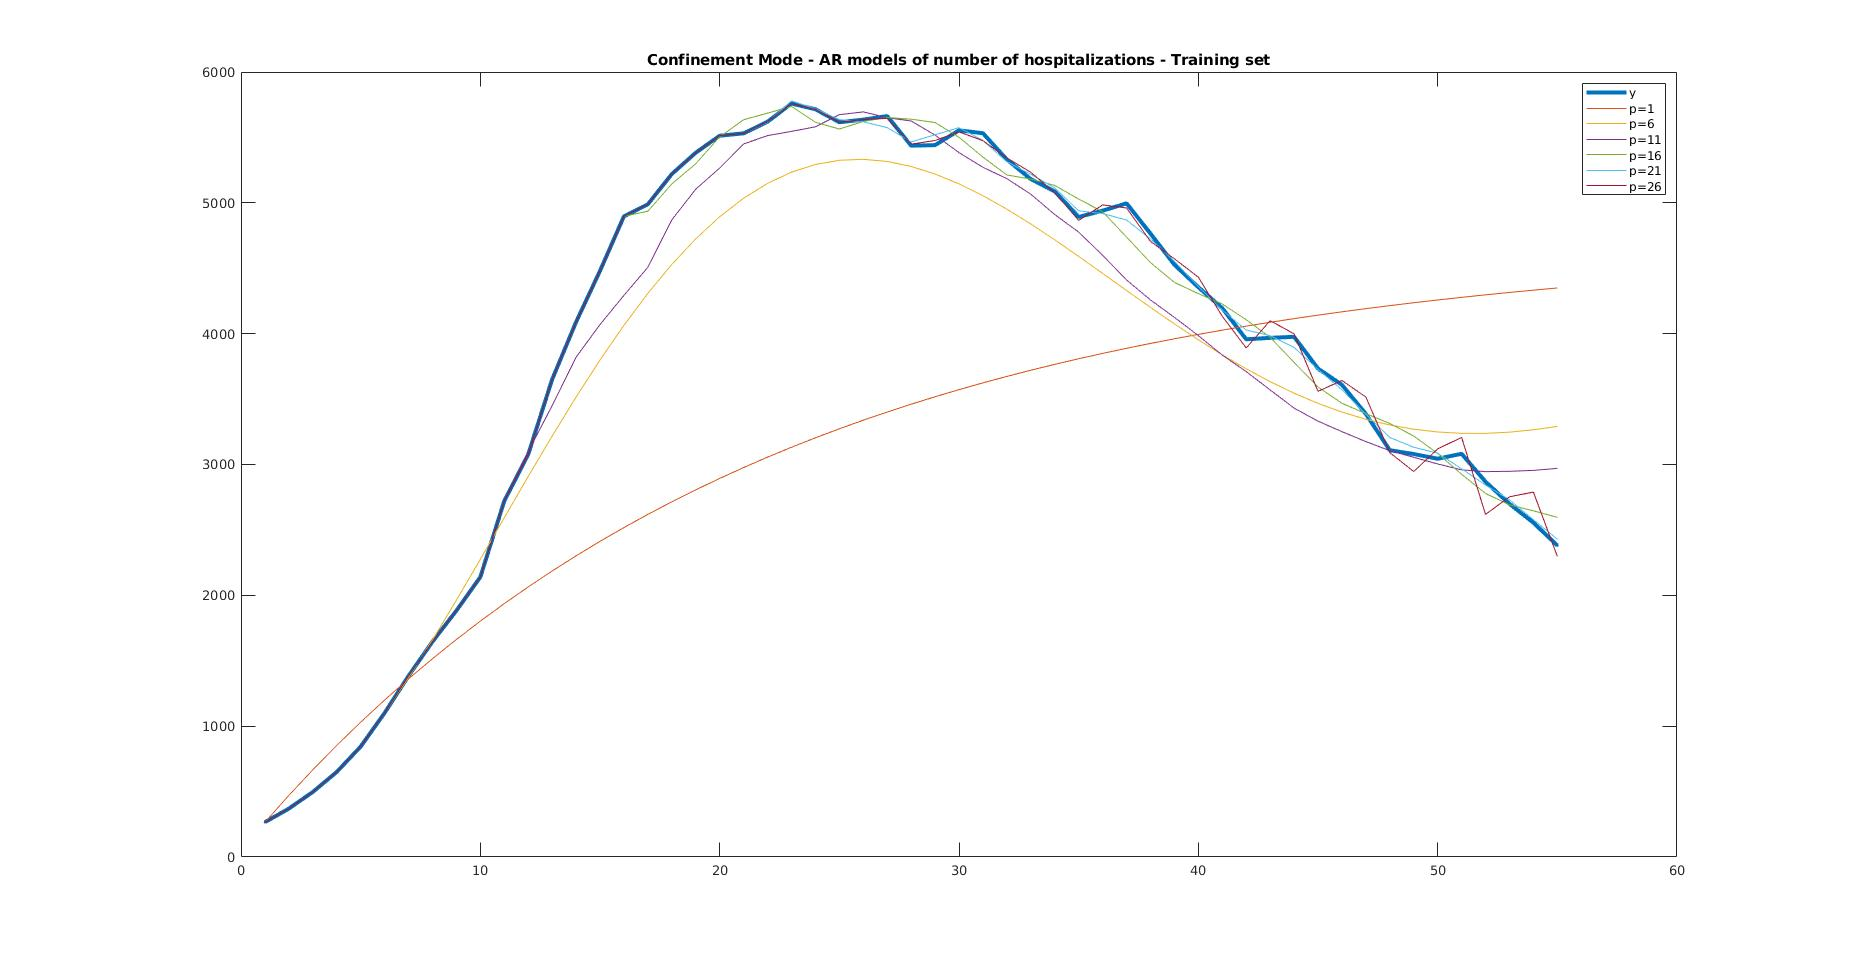
\includegraphics[scale=0.3]{Conf_train.jpg}
	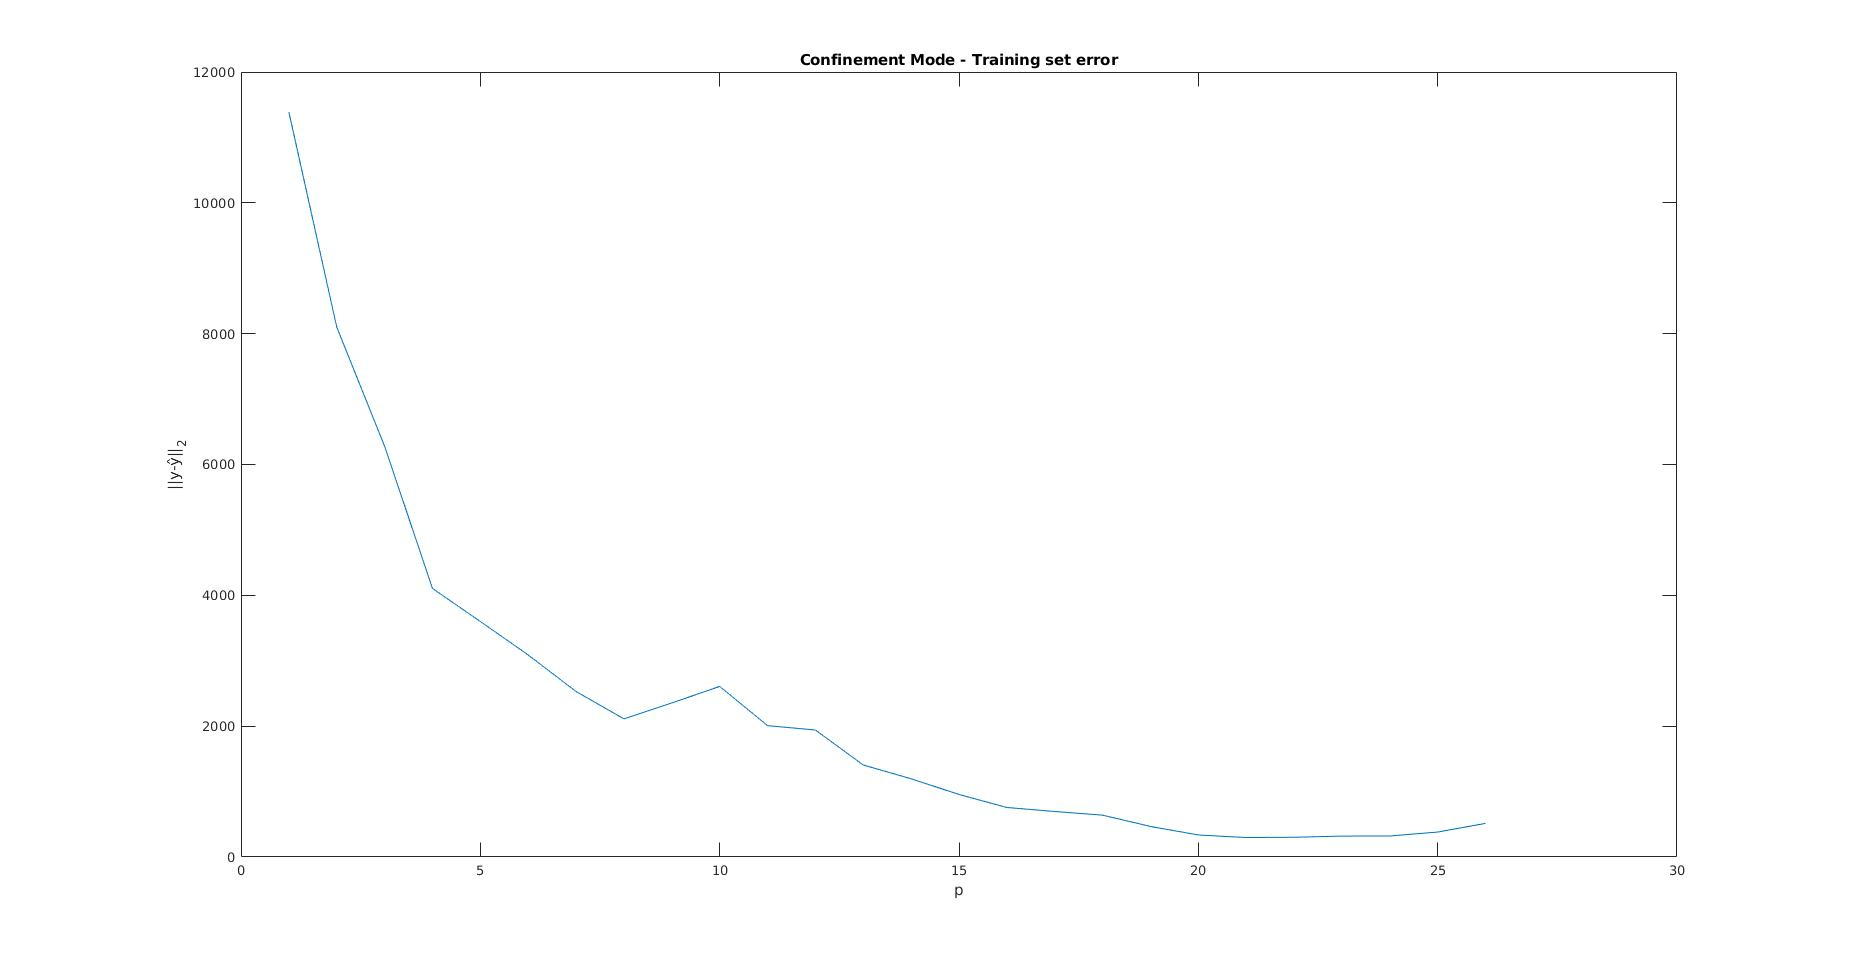
\includegraphics[scale=0.3]{Conf_Err_Train.jpg}
	\caption{Lockdown mode: training set predictions and error using the AR model, for different values of \(p\).}
	\label{fig:Conf_train}
\end{figure}

\begin{figure}[h!]
	\centering
	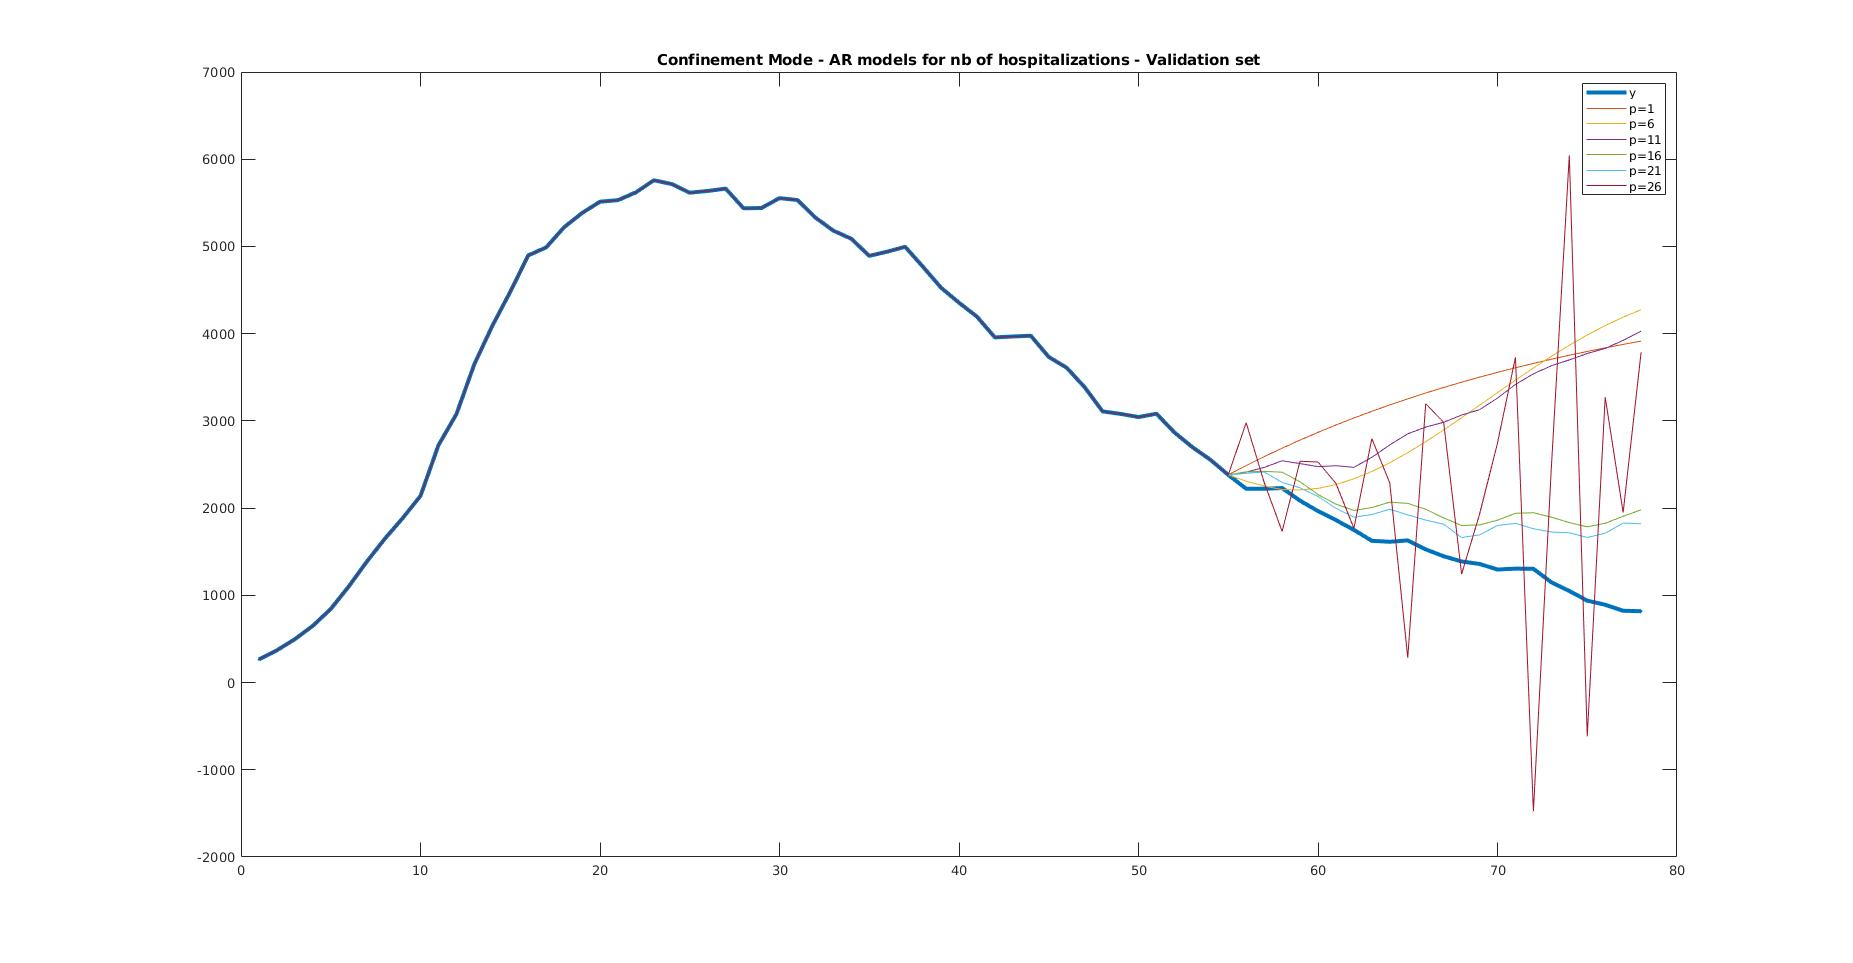
\includegraphics[scale=0.3]{Conf_val.jpg}
	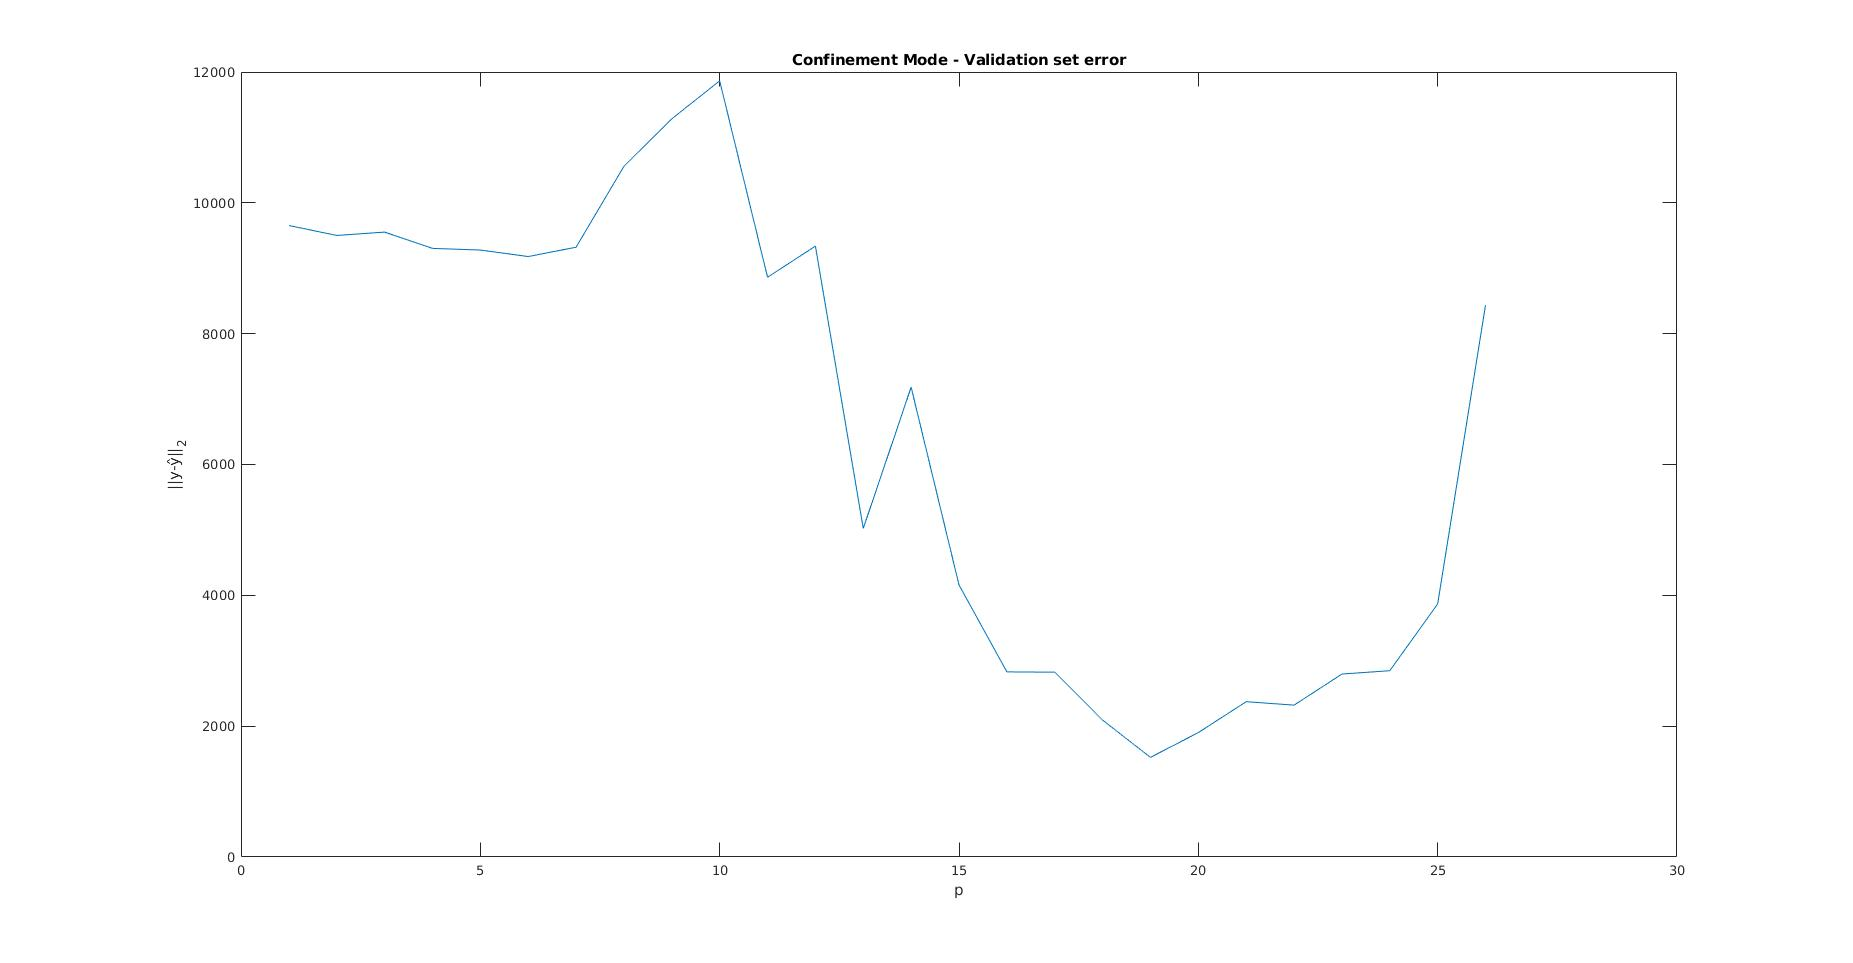
\includegraphics[scale=0.3]{Conf_Err_Val.jpg}
	\caption{Lockdown mode: validation set predictions and error using the AR model, for different values of \(p\).}
	\label{fig:Conf_val}
\end{figure}

\paragraph{Social distancing mode}
In the social distancing mode, we can make the same observations (in Figures~\ref{fig:SD_train} and \ref{fig:SD_val}) as in the previous mode: the error in the training set decreases when \(p\) increases except at some peaks.
For the validation set, we once again observe overfitting when \(p\) is higher than \(19\).
\begin{figure}[h!]
	\centering
	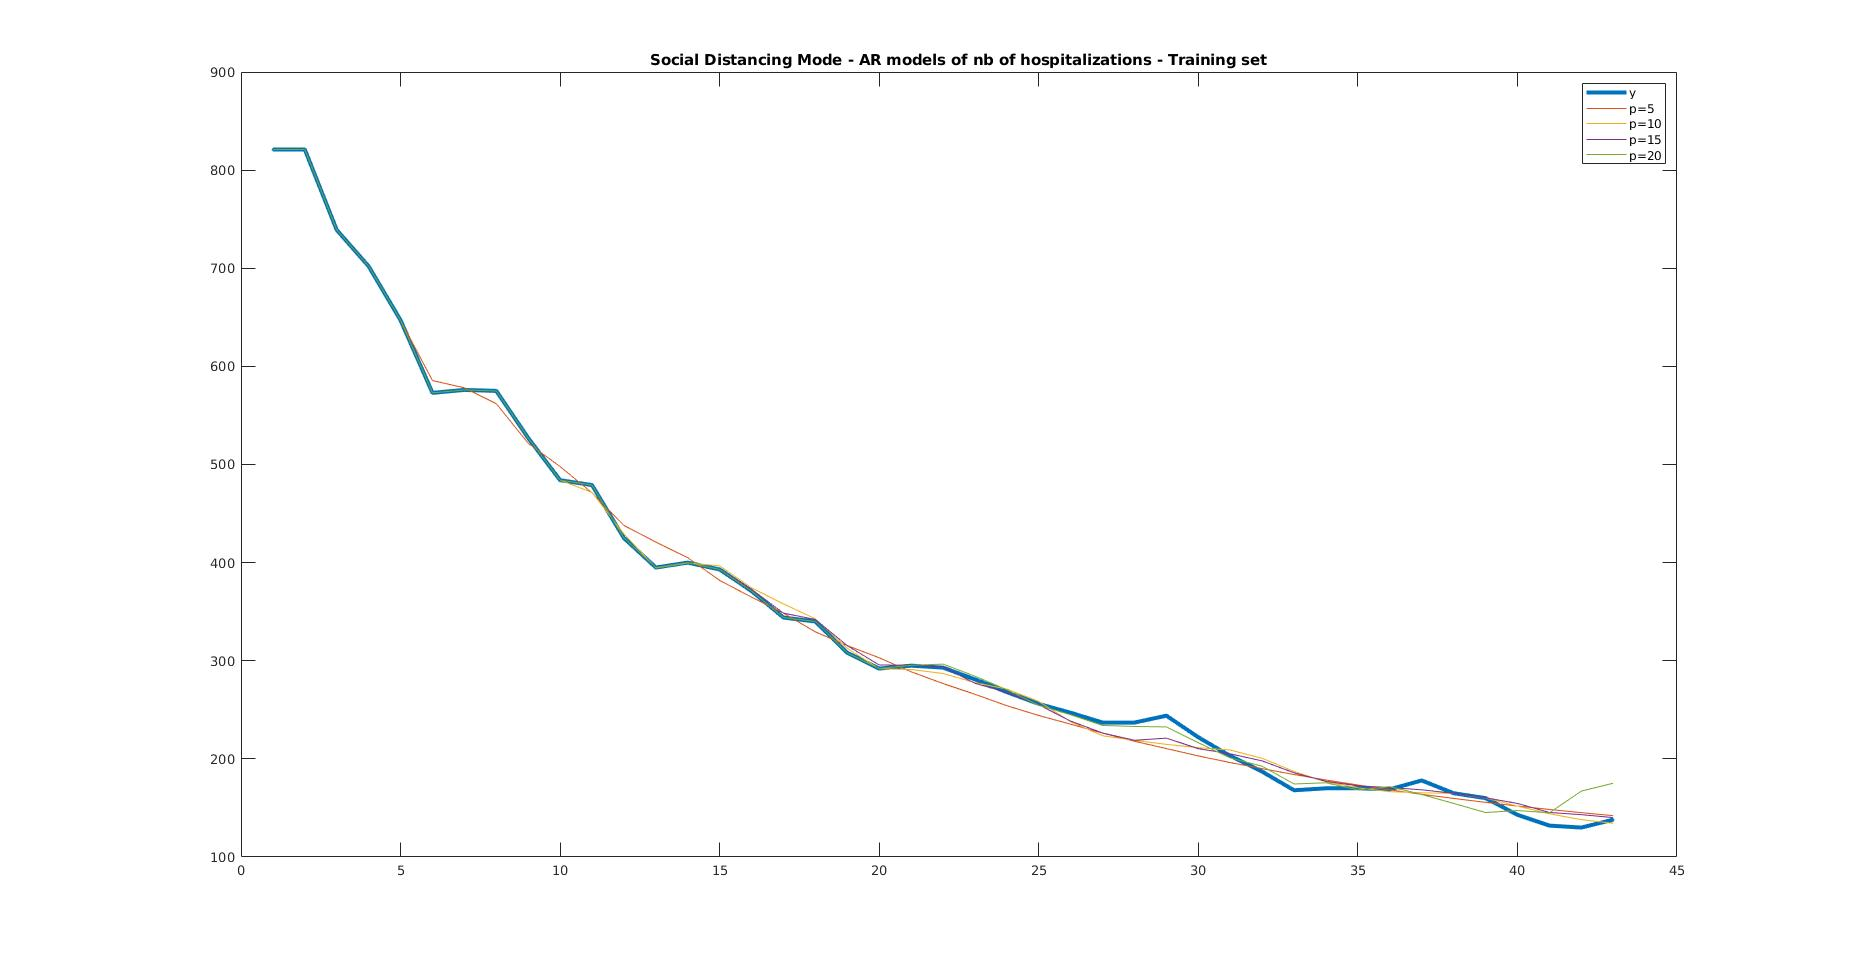
\includegraphics[scale=0.3]{SD_train.jpg}
	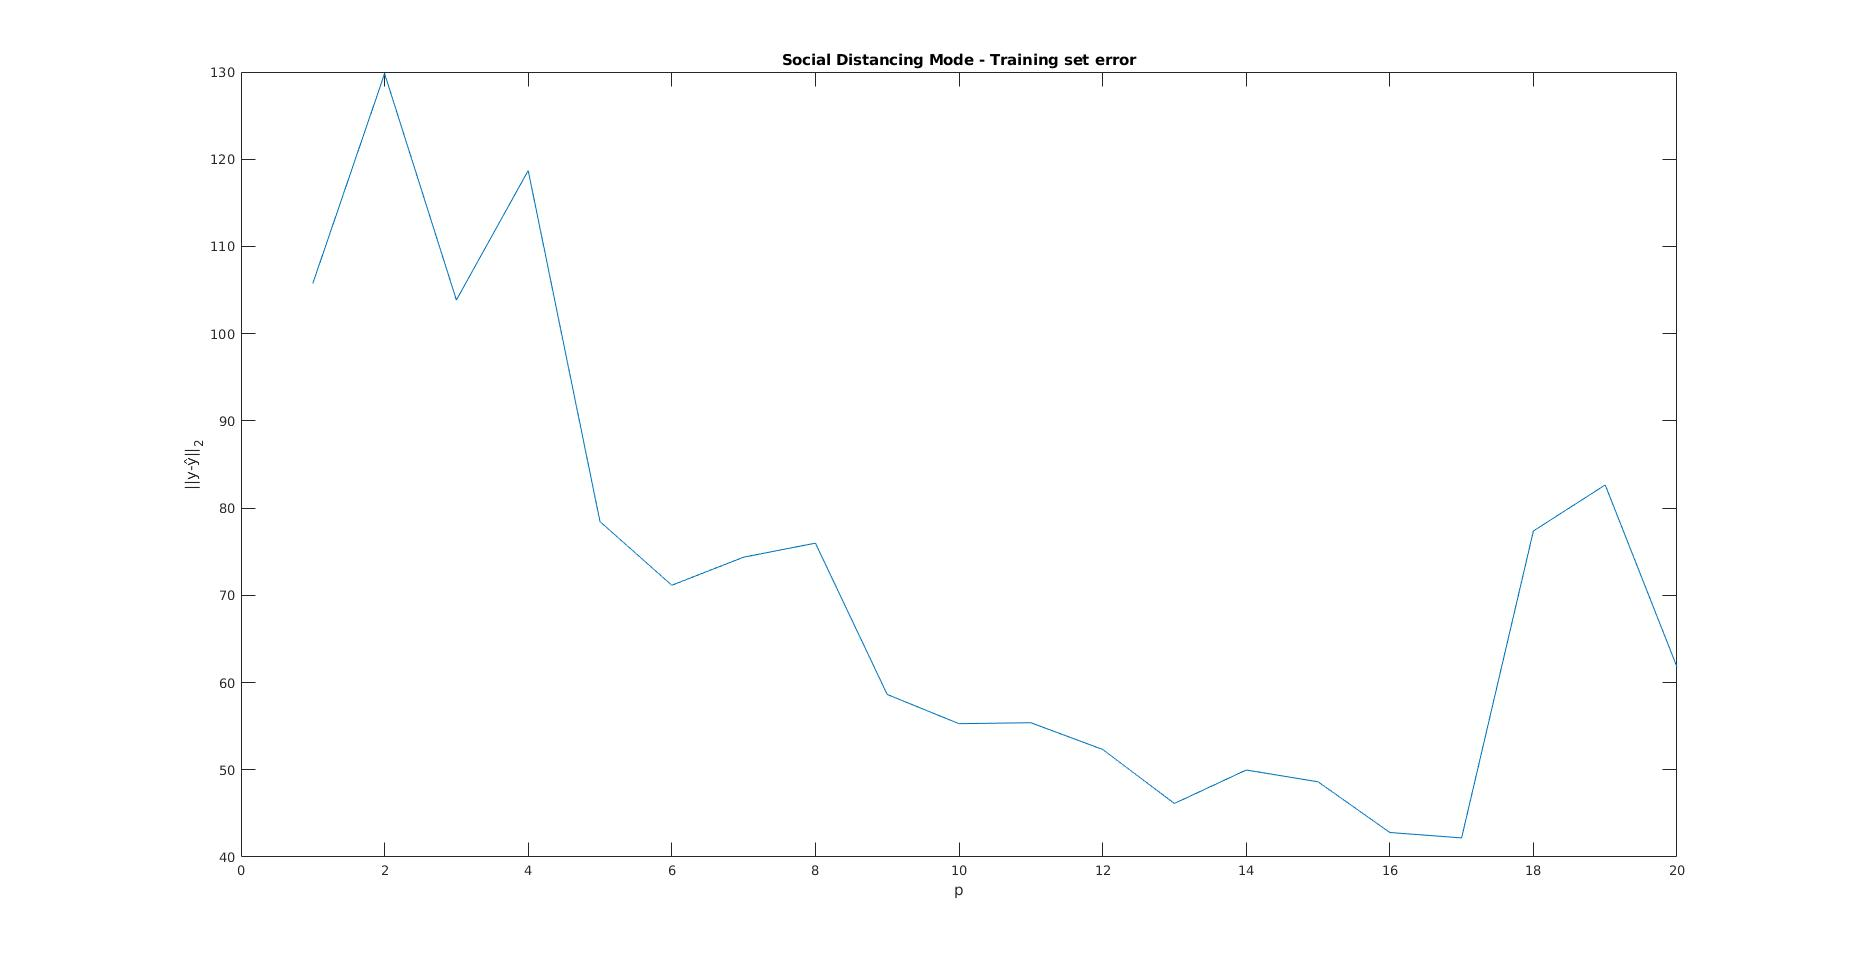
\includegraphics[scale=0.3]{SD_Err_Train.jpg}
	\caption{Social distancing mode: training set predictions and error using the AR model, for different values of \(p\).}
	\label{fig:SD_train}
\end{figure}

\begin{figure}[h!]
	\centering
	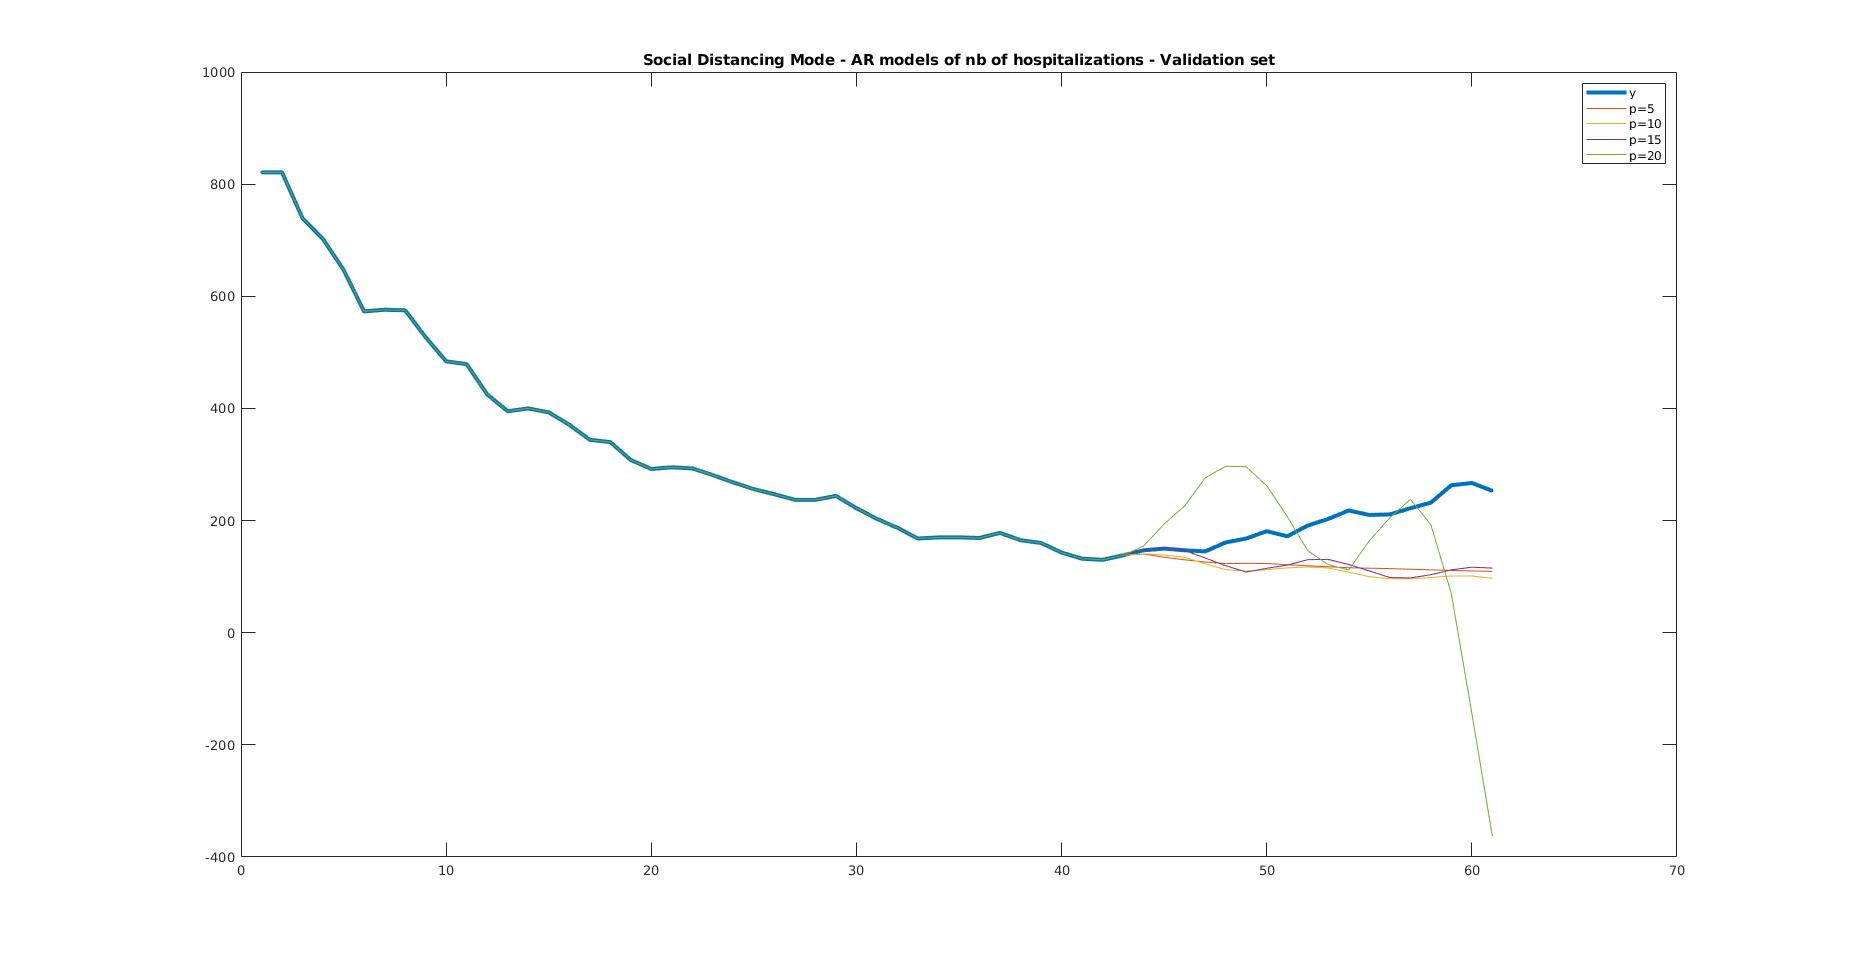
\includegraphics[scale=0.3]{SD_val.jpg}
	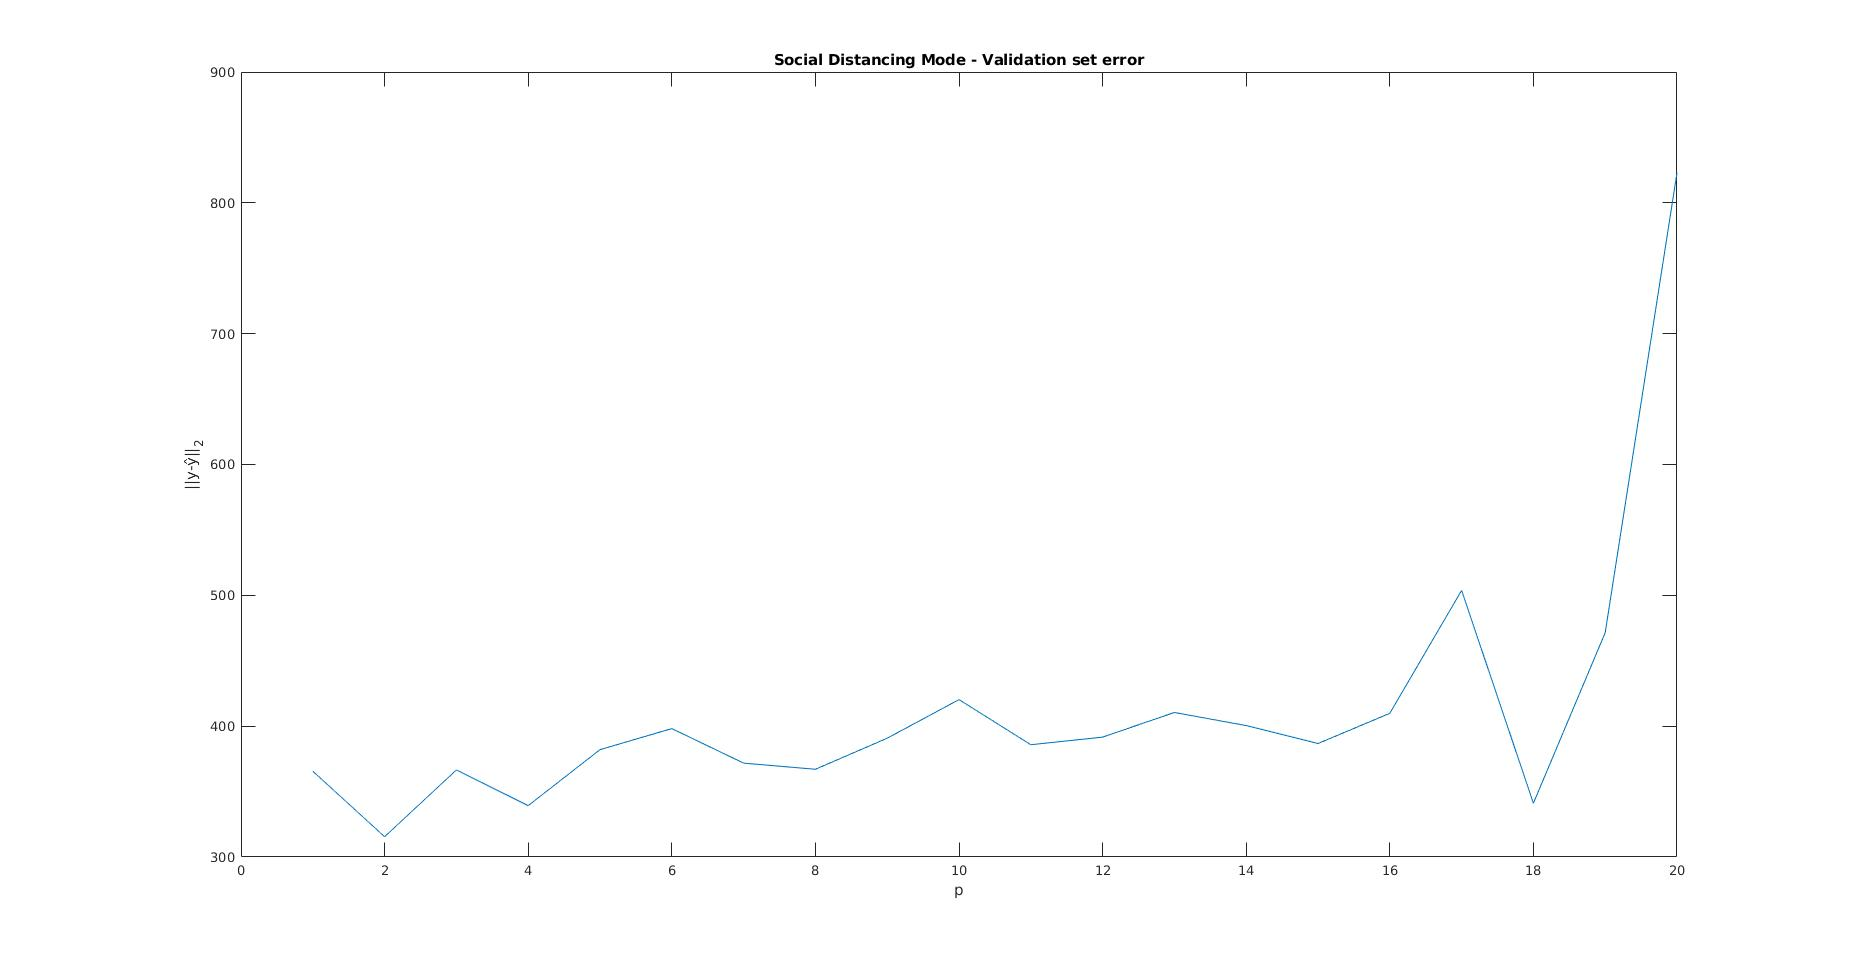
\includegraphics[scale=0.3]{SD_Err_Val.jpg}
	\caption{Lockdown mode: validation set predictions and error using the AR model, for different values of \(p\).}
	\label{fig:SD_val}
\end{figure}

\subsection*{Discussion}
In both modes, we have confirmed our intuition that the error in the training set should decrease. However, it is not monotonic and we still observe some peaks. One way to try to explain this is that when we solve the least squares problem, we minimize the error between the real values $y(t)$ and $\tilde{y}(t) = \alpha_0 + \sum_{i=1}^p \alpha_iy(t-i)$, that is, $e_1 = \snorm{y-\tilde{y}}$. However, when we compute the error on the training set, we consider $\hat{y}(t) = \alpha_0 + \sum_{i=1}^p \alpha_i \hat{y}(t-i)$, that is, $e_2 = \snorm{y-\hat{y}}$, and so we propagate the errors along with the time $t$. Clearly, this last error $e_2$ is bigger than the first one, $e_1$. Our intuition that the error should decrease monotonically can only apply to the error $e_1$ (which we have indeed observed in Figure~\ref{fig:e1}) and not to $e_2$.
\begin{figure}[h!]
	\centering
	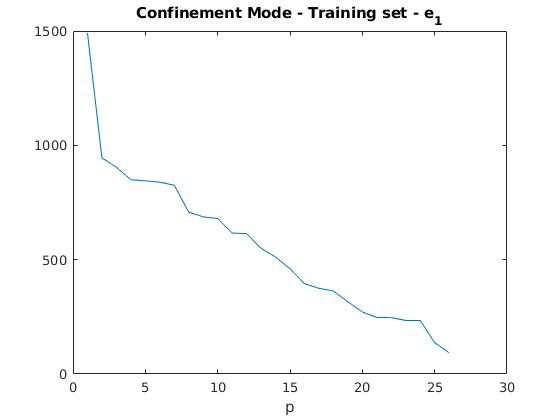
\includegraphics[scale=0.43]{Conf_train_e1.jpg}
	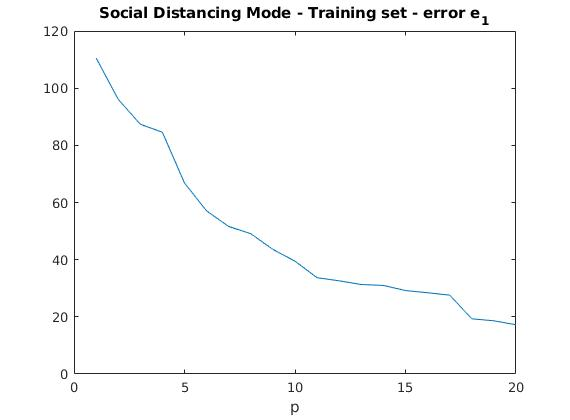
\includegraphics[scale=0.43]{SD_train_e1.jpg}
	\caption{The error $e_1$ monotonically decreases.}
	\label{fig:e1}
\end{figure}

Then, about the validation set errors, we can conclude that overfitting a training set does not yield good results for future predictions.

Note that in the analysis above, we only considered values of \(p\) such that the linear system of equations has more rows than columns.
In the case that we have more columns than rows, our system is underdetermined and so solving the system yields an infinity of solutions that are exact (if there are no linear combinations in the rows of course) which means that our training error is zero in theory (in practice, we have errors of order $10^{-4}$, for the confinement mode, and $10^{-9}$ for the social distancing mode, due to numerical imprecisions). As expected, we still have an overfitting that is visible in the validation set errors as they are very big for both modes.

\subsection*{Bonus question}
If we approximate the model in real time with data that we receive at fixed intervals, with our approach we will have to solve a new ``full-size'' least squares problem (as defined at the beginning of this section) everytime we want to include new data to improve the system. Indeed, we will have to add new rows each time we receive new data and solve it again. This can be expensive especially if the system is big.

That is why maintaining a real-time model with our approach to solve least squares problems is sub-optimal. It would be better if we could only consider the small changes without having to solve the whole system, for example by considering a recursive method to solve least squares problems.
\end{document}
